\documentclass{article}
\usepackage{graphicx}
\usepackage[margin=2cm]{geometry}

\title{\Huge \textbf{AppleStocks}\\\vspace{0.2em} \Large A Simple Application for Apple Stock Quotes Monitoring}
\author{
    Henrique Romão \\
    \textit{up202108067@up.pt}
    \and
    Mariana Bessa \\
    \textit{up202107946@up.pt}
}

\begin{document}

\maketitle

\begin{abstract}
    Escrever no fim
    % [TO-DO]
\end{abstract}

\section{Introduction}
This application was developed to provide users with a simple and intuitive way to view Apple stock quotes for a selected recent period. Users can customize their experience by choosing the time interval (in days or hours) and the duration of the interval, which can range from 2 to 10 intervals.

\section{Use Cases}

\begin{figure}
    \centering
    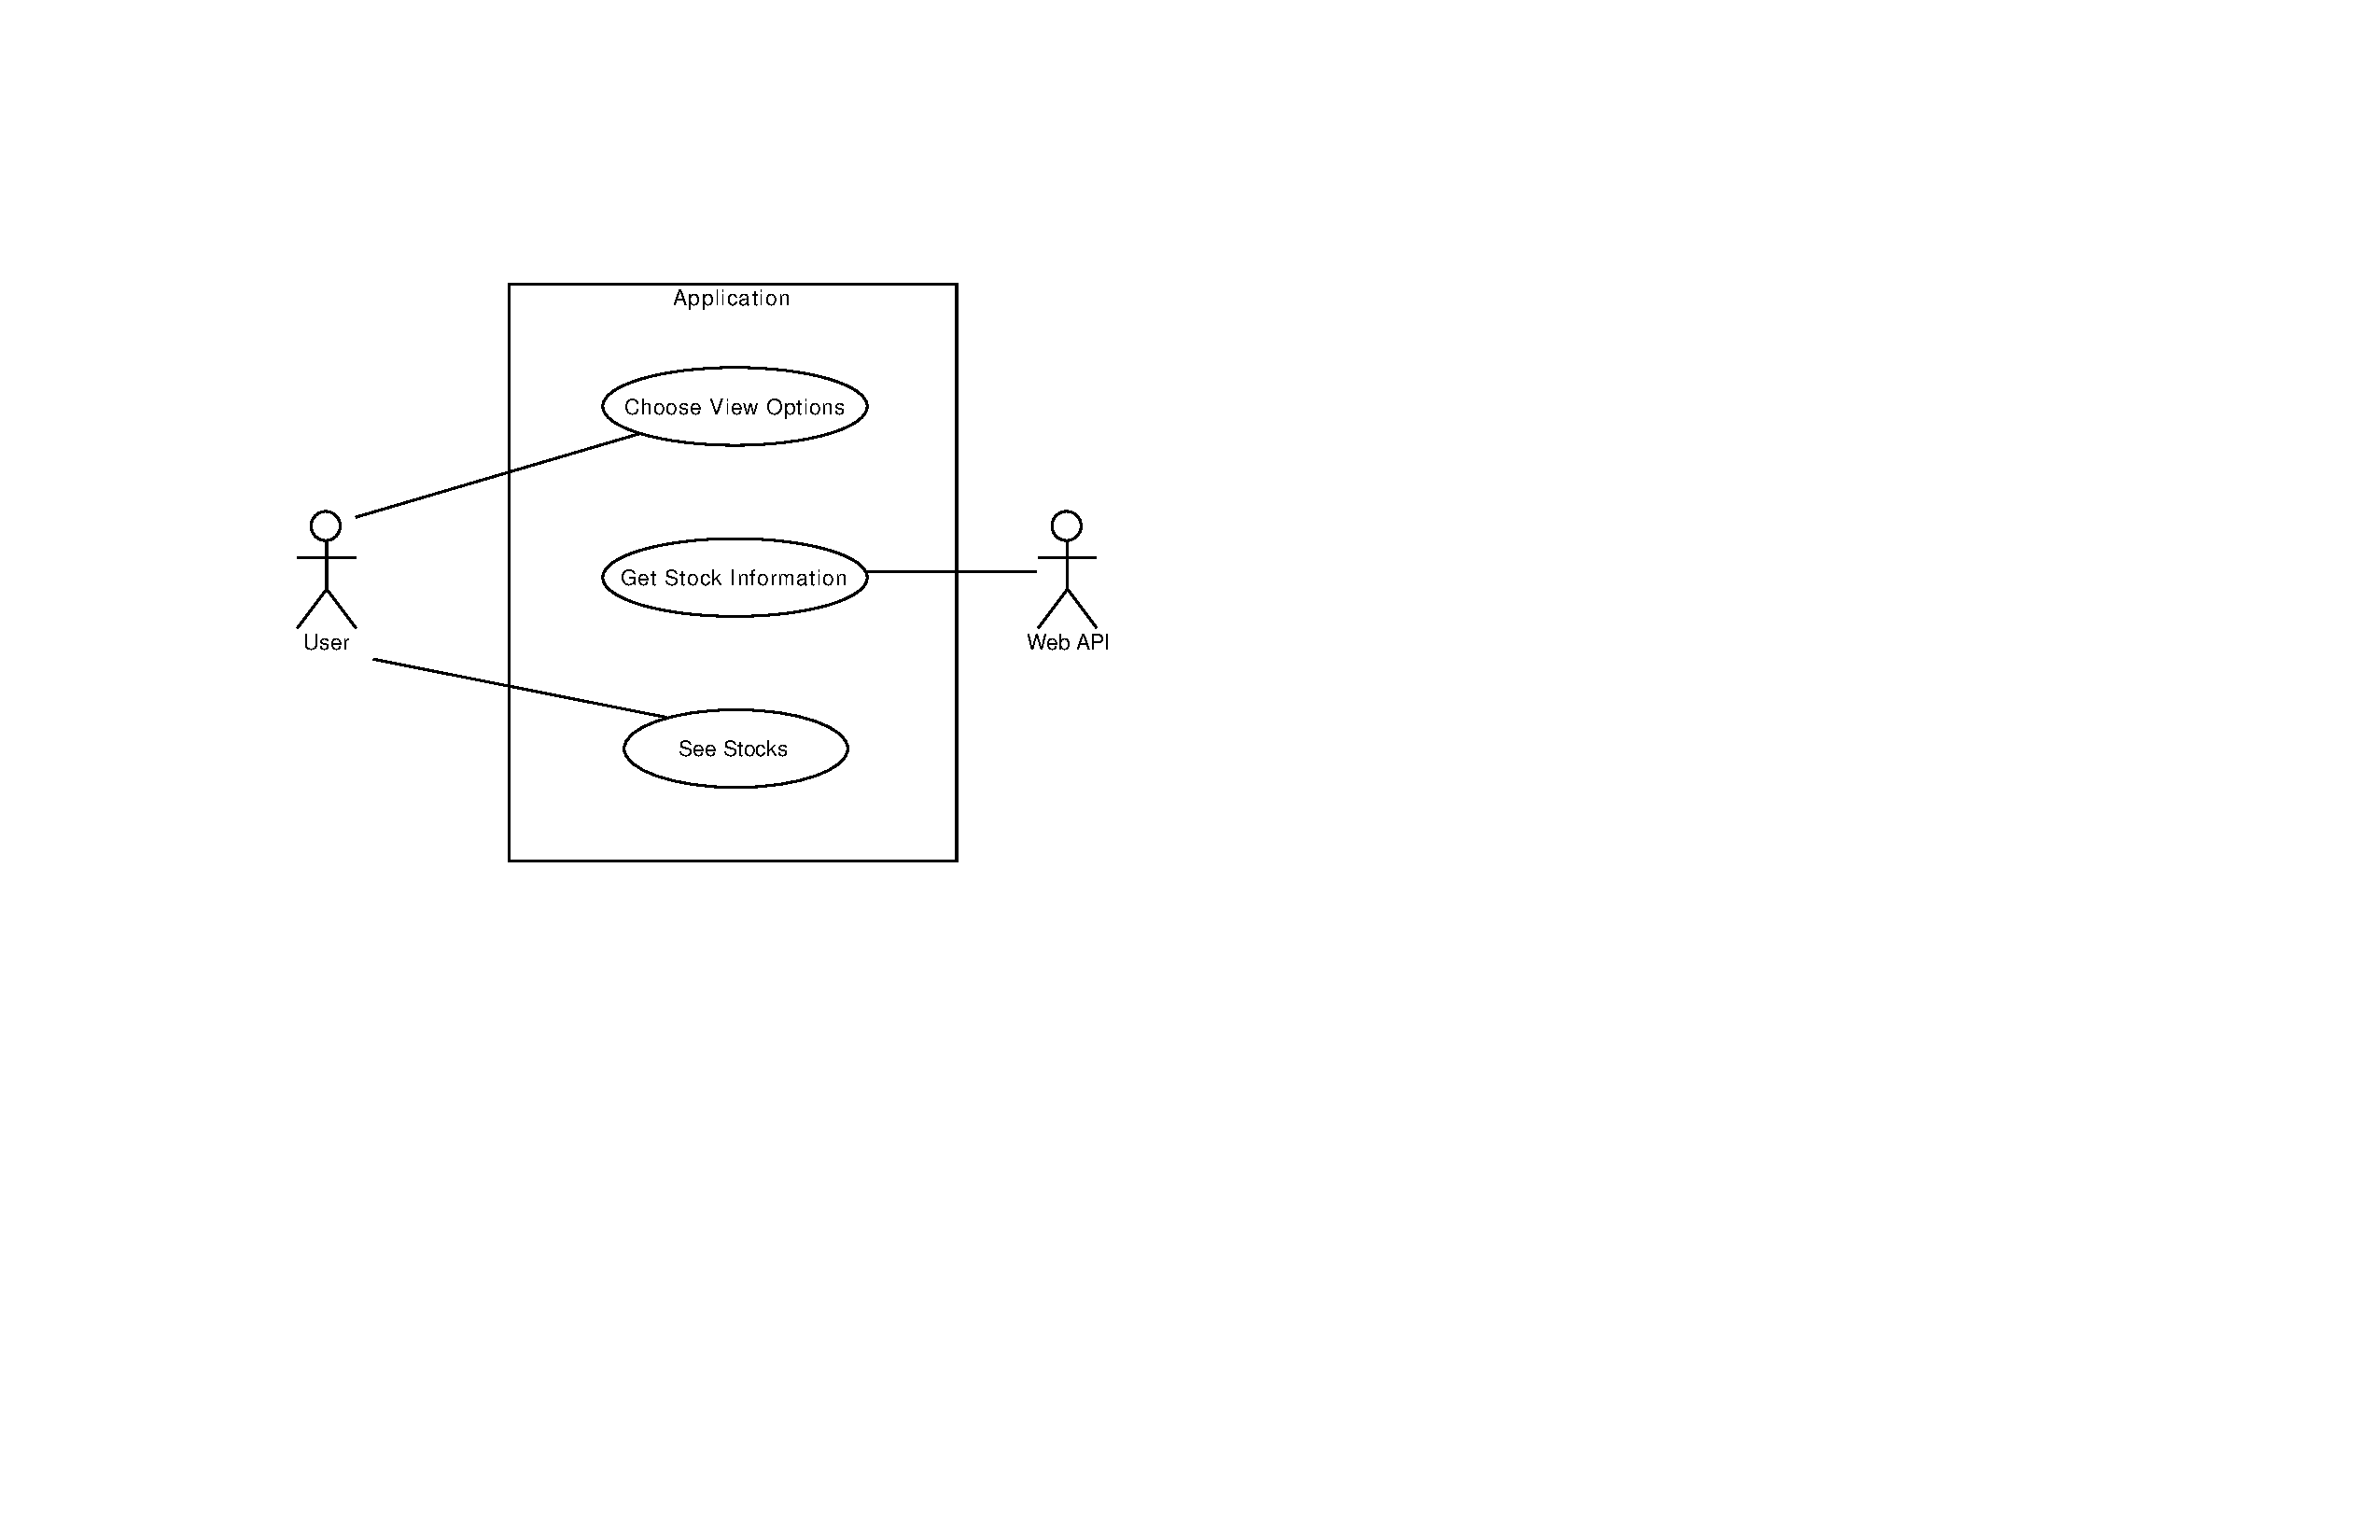
\includegraphics[width=0.6\linewidth]{Use Cases.pdf}
    \caption{Use Cases Diagram.}
    \label{fig:Use Cases}
\end{figure}

\section{Architecture}
This application was developed to provide users with a simple and intuitive way to view Apple stock quotes for a selected recent period. Users can customize their experience by choosing the time interval (in days or hours) and the duration of the interval, which can range from 2 to 10 intervals.

\subsection{Main Activity}

\subsection{Plot Activity}

\section{Interface}

\subsection{Main Activity}

\subsection{Plot Activity}


\section{User Experience}

\end{document}